\section{Existing applications}

We managed to find some applications, but also platforms allowing you to build your own application.

	\subsection{Bluebridge}
	Bluebridge is a provider of tourism applications. It provides :
	\begin{itemize}
		\item  Back-end technology (platform) to power your app
		\item  Mobile App Studio CMS (product) to design your app
		\item  Best-in-class app packages
		\item  Professional services
		\item  A message center to manage push notifications
	\end{itemize}

The platform is a Software as a service, using its own technology, so we don't have any way to know how they are implemented. But the features proposed on the website are interesting, so we will developp them.

\paragraph{GPS locating} As far as we thought, the GPS location is one of the main features when you want to implement an applications creating tours. Of course we can decide not to use it, and just display the best way between the monuments the user chose. This would mean that we assume that the user can find the first monument of the tour alone, and then will manage to find easily the way the application displays.
\begin{figure}[h!]
	\centering
	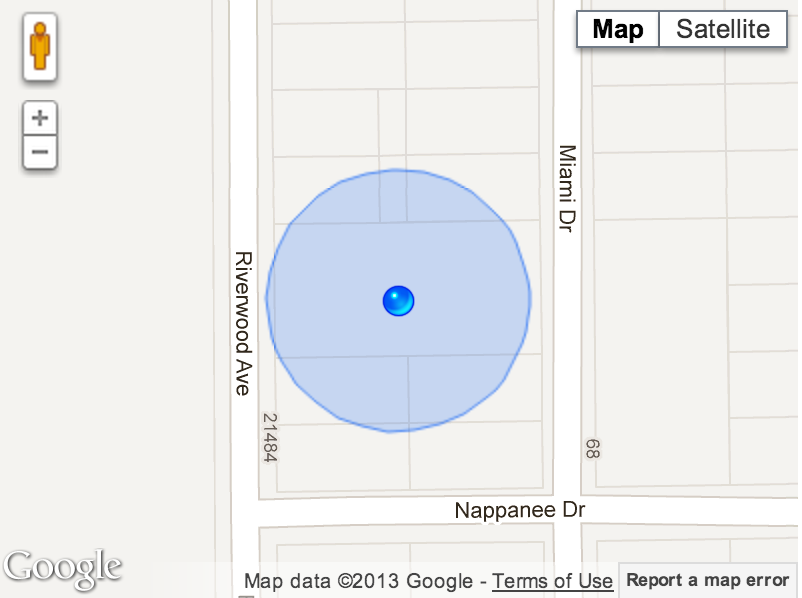
\includegraphics[scale=0.37]{input/current-location.png}
	\caption{Google Maps displaying your location.}
	\label{fig:location}
\end{figure}
The GPS location will allow the user to know where he is and to confirm he goes in the right direction.


\paragraph{GPS directions} This function is complementary with displaying the way between two monuments. Thanks to the GPS directions, the user can just be guided by the GPS, telling him which street he is currently in, where and when he should turn. Of course it will also announce his arrival to the monument he selected. It's not a compulsory feature, but it sure is a convenient one.
\begin{figure}[h!]
	\centering
	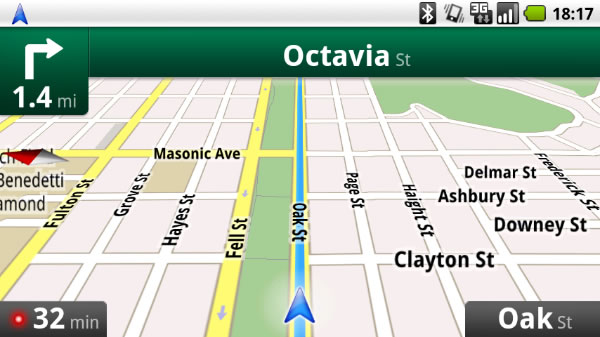
\includegraphics[width=0.6\textwidth]{input/directions.png}
	\caption{Google Maps displaying the navigation directions.}
	\label{fig:directions}
\end{figure}
Since Bluebridge is not a real application, those are the main features we found. They are pretty classic so we won't present them in other applications. Let's head to the second application.

\paragraph{Itinerary planner} It seems like the main idea of our application already exists. This feature is called Itinerary planner with Bluebridge, 

\subsection{mTrip}
